% !TeX TXS-program:compile = txs:///pdflatex/[--shell-escape]

\documentclass[11pt, letterpaper]{article}

\usepackage{minted}
\usepackage[utf8]{inputenc}
\usepackage[T1]{fontenc}
\usepackage{lmodern}
\usepackage{graphicx}
\usepackage{longtable}
\usepackage{wrapfig}
\usepackage{rotating}
\usepackage{amsmath}
\usepackage{textcomp}
\usepackage{amssymb}
\usepackage{hyperref}
\usepackage[spanish]{babel}
\usepackage[round]{natbib}
\usepackage{subcaption}


\title{\bfseries Tarea}
\author{Ángel García Báez}
\date{\today}
\setcounter{tocdepth}{3} 

\begin{document}
	
	% Página de presentación
	\begin{titlepage}
		\centering
		
\includegraphics[width=0.2\textwidth]{logo.png}\par
		\vspace{1cm}
		{\LARGE \bfseries Universidad Veracruzana \par}
		\vspace{1cm}
		{\Large Maestría en Inteligencia Artificial\par}
		\vspace{3cm}
		{\LARGE \bfseries Visión por Computadora \par}
		\vspace{1cm}
		{\Large \bfseries Tarea 3. Implementación de la ecualización de pixeles por histograma para el mejoramiento de imágenes en Julia. \par}
		\vfill
		{\Large \textit{Ángel García Báez}\par}
		\vspace{1cm}
		{\Large Profesor: Dr. Héctor Acosta Mesa\par}
		\vfill
		{\Large \today \par}
	\end{titlepage}
	
	% Página exclusiva para la tabla de contenidos
	\newpage
	\tableofcontents
	\newpage
	
	% Sección para el problema 1
	\section{Objetivo de la práctica}
	
Se tiene un conjunto de 4 imágenes que en esencia, son la misma imagen pero variaciones en sus tonalidades de grises:

\begin{figure}[h!]
	\centering
	\begin{minipage}{0.45\textwidth}
		\centering
		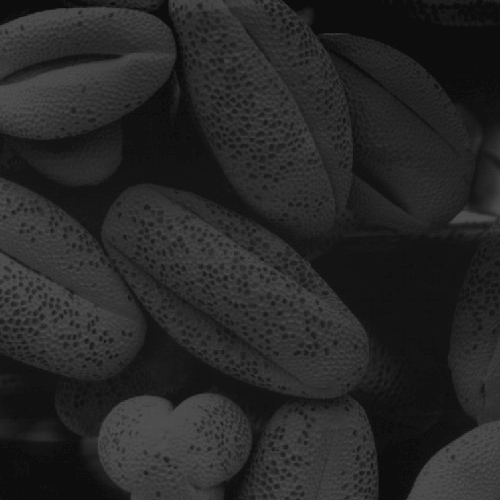
\includegraphics[width=\textwidth]{IMG/Fig3.15(a)1.jpg}
		\caption{Imagen oscurecida.}
		\label{fig:f1}
	\end{minipage}\hfill
	\begin{minipage}{0.45\textwidth}
		\centering
		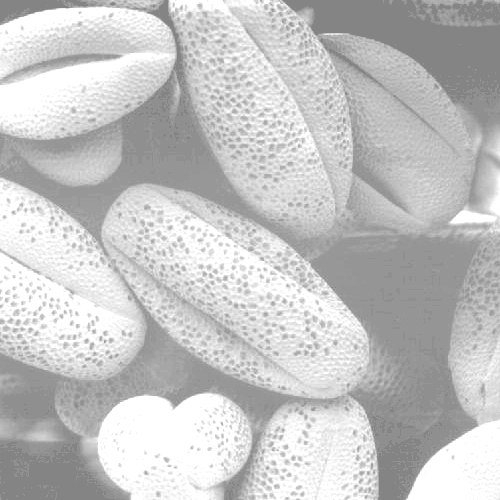
\includegraphics[width=\textwidth]{IMG/Fig3.15(a)2.jpg}
		\caption{Imagen opaca.}
		\label{fig:f2}
	\end{minipage}
	
	\vskip\baselineskip
	
	\begin{minipage}{0.45\textwidth}
		\centering
		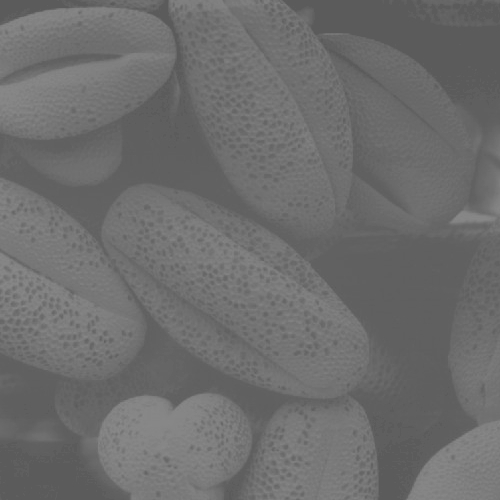
\includegraphics[width=\textwidth]{IMG/Fig3.15(a)3.jpg}
		\caption{Imagen opaca oscura.}
		\label{fig:f3}
	\end{minipage}\hfill
	\begin{minipage}{0.45\textwidth}
		\centering
		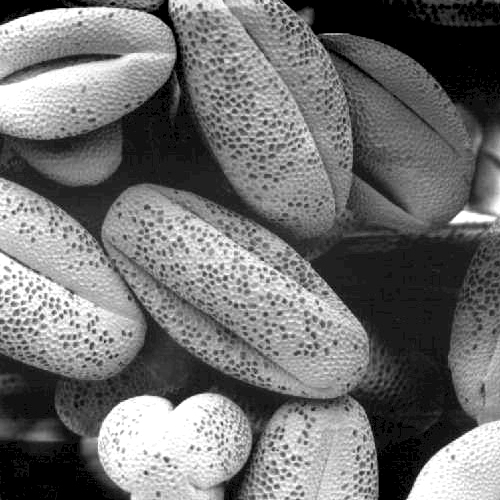
\includegraphics[width=\textwidth]{IMG/Fig3.15(a)4.jpg}
		\caption{Imagen balanceada.}
		\label{fig:f4}
	\end{minipage}
	\caption{Figuras de interés extraídas del libro de Digital Image Processing.}
	\label{fig:4images}
\end{figure}

El objetivo de la presente practica es implementar un algoritmo basado en el histograma de los pixeles de a imagen con la finalidad de ecualizar la imagen y conseguir un mejoramiento de la misma de forma que se puedan comparar los resultados arrojados para cada imagen.

Para ello, se pide que:

\begin{enumerate}
	\item Escribir un programa que haga el computo del histograma de la imagen
	\item Implementación de la técnica de ecualización por histograma que se discutió en la sección 3.3.1.
	\item  Usar el conjunto de figuras propuestas y aplicarles la técnica de ecualización implementada.
	
	\item  Para cada una de las imágenes se debe incluir como mínimo, la imagen original, su histograma, la imagen mejorada por la técnica y su correspondiente histograma
	
	\item  Explique brevemente porque el resultado de la imagen fue el obtenido y como es que mejoro.
	
\end{enumerate}
	
	\newpage
	
	\section{Metodología}
	
	Para la construcción del histograma, se plantea reallizar el conteo de frecuencias de cada uno de los valores de los pixeles que se encuentran en un rango entre 0 y 255.
	
	Posteriormente, se gráfica tomando de base la estructura del gráfico de barras.
	
	Para la obtención de las probabilidades de cada valor en el rango, se calcula como sigue segun lo revisado en \cite{depaoli2012} y \cite{gonzalez2018digital}:
	
	$$P_k = \frac{ n_k}{n} $$
	
	Donde:

	\begin{itemize}
		\item $P_k = $ Probabilidad del nivel $k-ésimo$ de gris.
		\item $n_k = $ Cantidad de pixeles de nivel gris $k$.
		\item $n = $ Cantidad total de pixeles.
	\end{itemize}
	
	Posteriormente, para lograr la expansión del rango se utiliza la distribución de probabilidad acumulada, definida por:
	
	$$F(k) = \sum^{k}_{i=0}{P_i} \text{ para } 0 \leq k \leq 255$$
	
	Aplicada sobre la expansión del caso, se utiliza junto con la siguiente normalización, contando con el caso donde el mínimo de la distribución no sea 0.
	
	$$G(k)  = 255 * \frac{F(k) - min(F) }{255-min(F)}$$
	
	Donde:
	
	\begin{itemize}
		\item $F = $ Es el conjunto de valores de toda la distribución acumulada.
		\item $F(k) = $ Es la probabilidad acumulada hasta el pixel $k-ésimo$.
	\end{itemize}
	
	Dado el conjunto de imágenes, se plantea implementar el filtro en lenguaje Julia haciendo uso de sus módulos para operar con imágenes como matrices, dada su simpleza y velocidad.

	
\newpage
	
\section{Resultados}

A continuación se muestran los resultados obtenidos para cada una de las figuras:

\subsection{Figura 1}


	
\begin{figure}[h]
		\centering
		\begin{minipage}{0.45\textwidth}
			\centering
			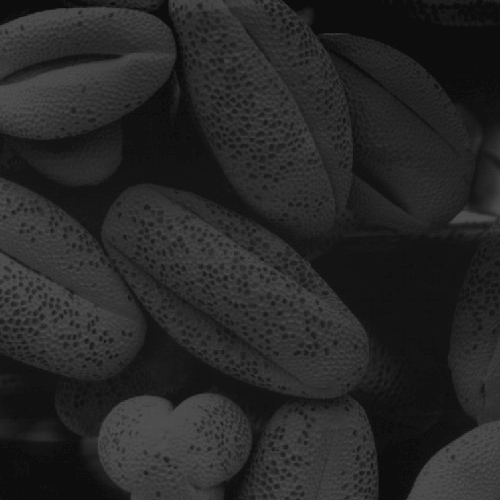
\includegraphics[width=\textwidth]{IMG/Fig3.15(a)1.jpg}
			\caption{Figura 1 original.}
			\label{fig:f5}
		\end{minipage}\hfill
		\begin{minipage}{0.45\textwidth}
			\centering
			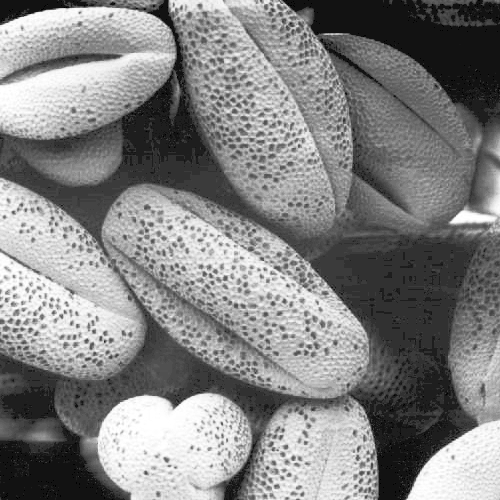
\includegraphics[width=\textwidth]{RESULTADOS/img15.png}
			\caption{Figura 1 mejorada.}
			\label{fig:f6}
		\end{minipage}
		
		\vskip\baselineskip
		
		\begin{minipage}{0.5\textwidth}
			\centering
			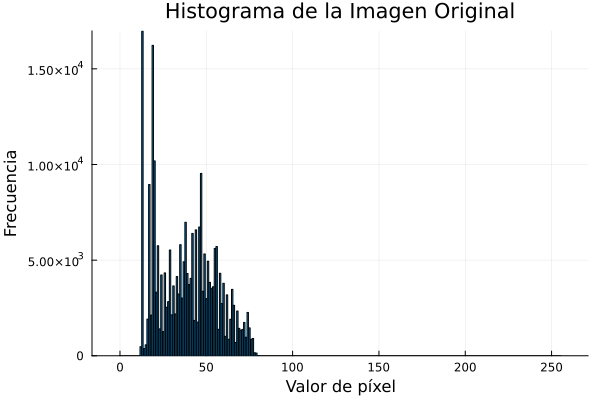
\includegraphics[width=\textwidth]{RESULTADOS/img11.png}
			\caption{Histograma original.}
			\label{fig:f7}
		\end{minipage}\hfill
		\begin{minipage}{0.5\textwidth}
			\centering
			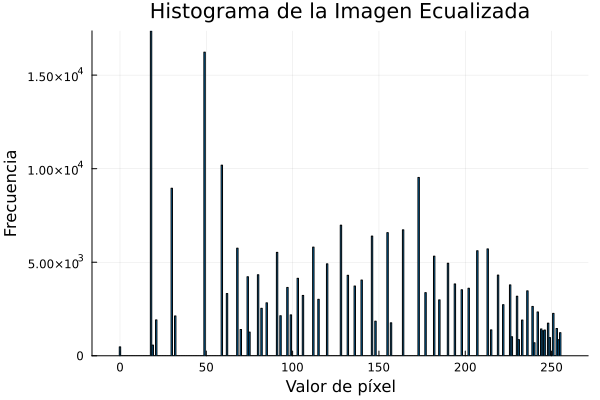
\includegraphics[width=\textwidth]{RESULTADOS/img13.png}
			\caption{Histograma ecualizado.}
			\label{fig:f8}
		\end{minipage}
		\caption{Comparativa de resultados para la figura 1.}
		\label{fig:R1}
	\end{figure}

Acorde con el histograma de la figura 1 original, se puede apreciar como es que la mayoria de sus pixeles se encuentra a la izquierda del histograma, es decir, que su rango de grises son mayormente oscuros casi siendo negros.

Al aplicar el mejoramiento de la imagen, se observa como dicho comportamiento del histograma  pasa de estar concentrado a la izquierda para poder expandirse a lo largo de todo el rango de grises, reflejandose esto mismo en la imagen que presenta matices más claros con tonalidades de blanco.

	\begin{figure}[h]
	\centering
	\begin{minipage}{0.45\textwidth}
		\centering
		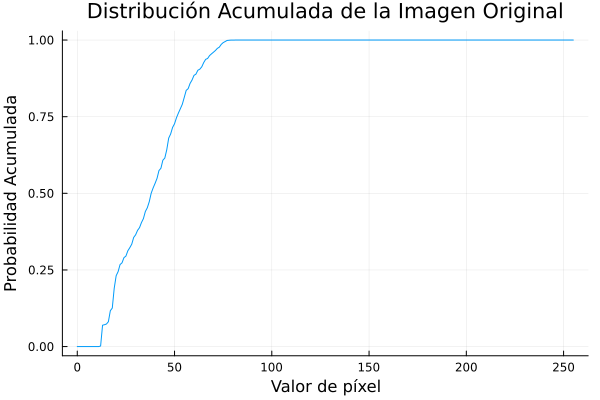
\includegraphics[width=\textwidth]{RESULTADOS/img12.png}
		\caption{Distribución acumulada original.}
		\label{fig:f9}
	\end{minipage}\hfill
	\begin{minipage}{0.45\textwidth}
		\centering
		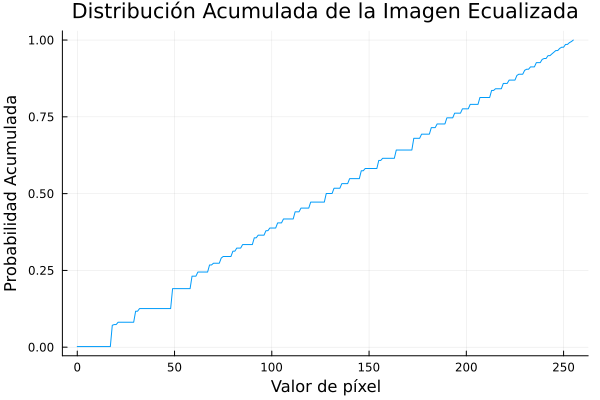
\includegraphics[width=\textwidth]{RESULTADOS/img14.png}
		\caption{Distribución acumulada ecualizada.}
		\label{fig:f10}
	\end{minipage}
	
	\caption{Comparativa de distribuciones acumuladas para la figura 1.}
	\label{fig:R2}
\end{figure}

Adicionalmente, se gráfico la función de probabilidad acumulada para los pixeles. Se puede observar como la función de probabilidad asociada a la figura 1 original tiende a crecer rapidamente hasta alcanzar su máximo en valores cerca del 100, evidenciando la fuerte carga de los tonos de gris en los pixeles hacia tonos oscuros.

Por otro lado, la gráfica correspondiente a la figura 1 mejorada se observa como si fuera una linea casi diagonal con ligeras perturbaciones en su camino.
Resalta en dicha gráfica que la mayor cantidad de perturbaciones se encuentran justamente en los valores de pixeles comprendidos entre 0 y 100, mostrando así como mantiene su relación respecto a la gráfica de la imagen original pero expandiendo el rango de valores que pueden tomar los pixeles.


\newpage

	
 \subsection{Figura 2}

\begin{figure}[h]
	\centering
	\begin{minipage}{0.45\textwidth}
		\centering
		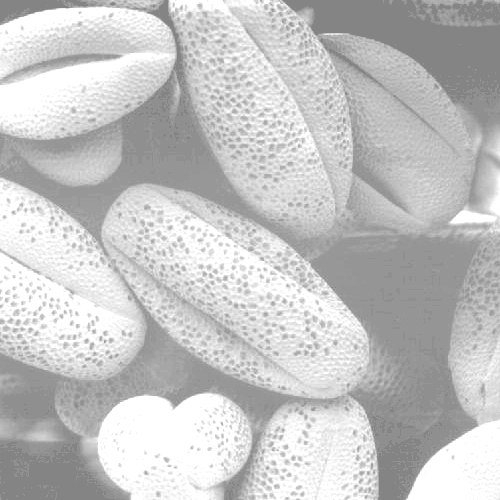
\includegraphics[width=\textwidth]{IMG/Fig3.15(a)2.jpg}
		\caption{Figura 2 original.}
		\label{fig:f11}
	\end{minipage}\hfill
	\begin{minipage}{0.45\textwidth}
		\centering
		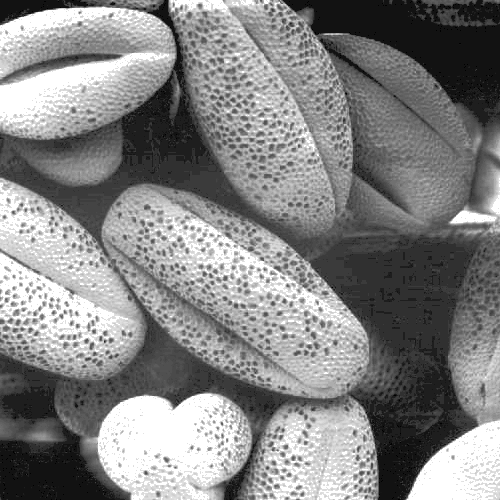
\includegraphics[width=\textwidth]{RESULTADOS/img25.png}
		\caption{Figura 2 mejorada.}
		\label{fig:f12}
	\end{minipage}
	
	\vskip\baselineskip
	
	\begin{minipage}{0.5\textwidth}
		\centering
		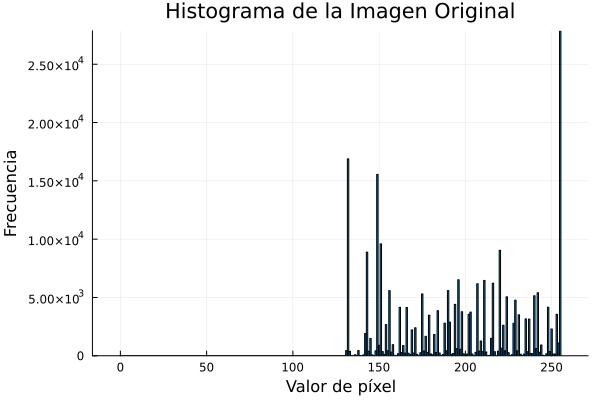
\includegraphics[width=\textwidth]{RESULTADOS/img21.png}
		\caption{Histograma original.}
		\label{fig:f13}
	\end{minipage}\hfill
	\begin{minipage}{0.5\textwidth}
		\centering
		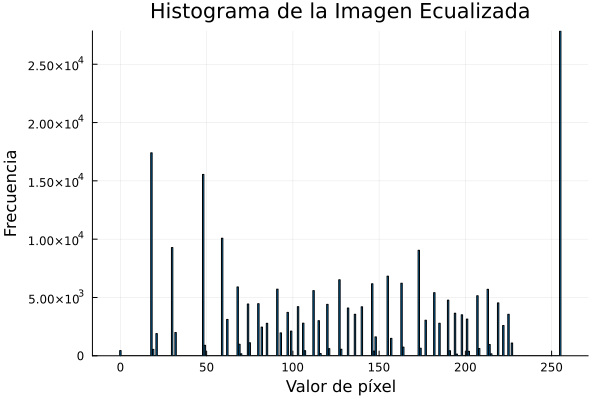
\includegraphics[width=\textwidth]{RESULTADOS/img23.png}
		\caption{Histograma ecualizado.}
		\label{fig:f14}
	\end{minipage}
	\caption{Comparativa de resultados para la figura 2.}
	\label{fig:R3}
\end{figure}

La imagen 2 se caracteriza principalmente por tener tonalidades opacas, dicho comportamiento se refleja en el histograma original, puesto que sus frecuencias caen totalmente en valores a la derecha del gráfico, por encima de los valores de 100.

La imagen mejorada logra ampliar el rango de los pixeles de la imagen original al punto que se logra distinguir perfectamente entre los tonos, aunque parecieria igual a la figura mejorada 1, el histograma asociado muestra que si bien, se realizo una expansión del rango de valores de los pixeles, existe una fuerte carga hacia el color blanco y aun así, se abarca la mayoría de los valores pero no el espectro en su totalidad.

\begin{figure}[htbp]
	\centering
	\begin{minipage}{0.45\textwidth}
		\centering
		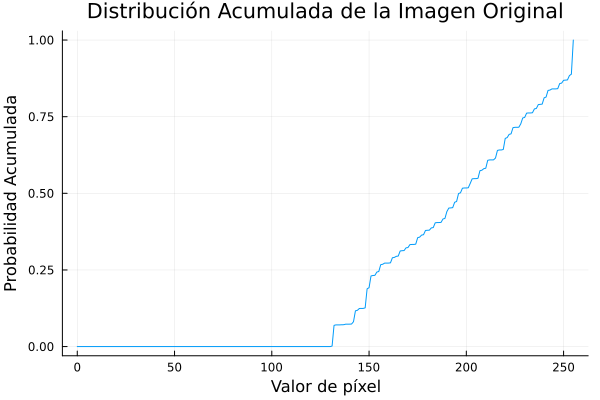
\includegraphics[width=\textwidth]{RESULTADOS/img22.png}
		\caption{Distribución acumulada original.}
		\label{fig:f15}
	\end{minipage}\hfill
	\begin{minipage}{0.45\textwidth}
		\centering
		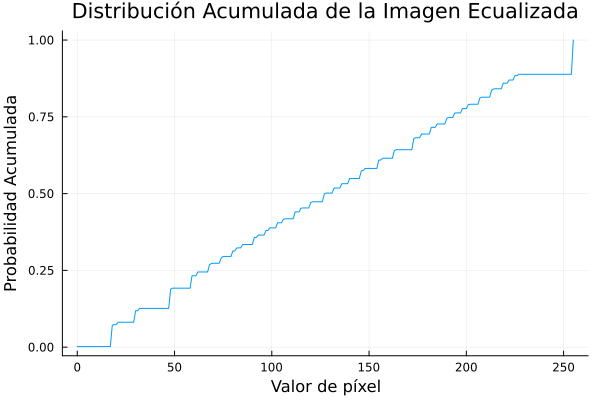
\includegraphics[width=\textwidth]{RESULTADOS/img24.png}
		\caption{Distribución acumulada ecualizada.}
		\label{fig:f16}
	\end{minipage}
	
	\caption{Comparativa de distribuciones acumuladas para la figura 2.}
	\label{fig:R4}
\end{figure}

Complementariamente se obtuvo la distribución de probabilidad acumulada de la figura 2, misma que muestra un comportamiento inverso al de la figura 1. Dicha gráfica refleja como no existen pixeles con vaores de entre 0 y 120, despues del 120 se observa como la probabilidad se va acumulando gradualmente hasta que llega a dar un salto marcado en el valor 255.

Dicho comportamiento se logra reducir en la distribución de probabilidad acumulada de la imagen mejorada, la cual se presenta en su mayoria como si fuera una diagonal con leves perturbaciones en su trayecto, pero es notorio como dicha gráfica tiene un comportamiento lleno de perturbaciones en los valores de 0 a 50 y de 230 a 255, es decir, en los extremos.

\newpage

\subsection{Figura 3}

\begin{figure}[h]
	\centering
	\begin{minipage}{0.45\textwidth}
		\centering
		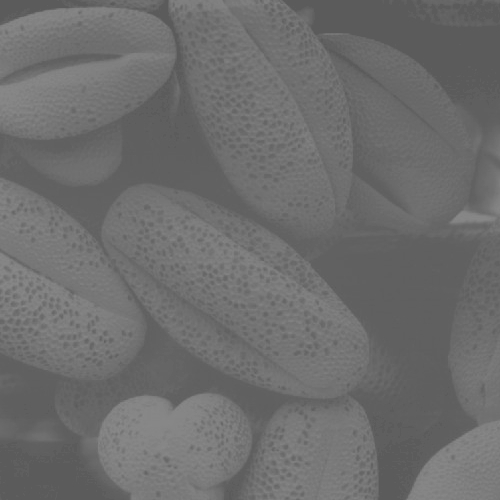
\includegraphics[width=\textwidth]{IMG/Fig3.15(a)3.jpg}
		\caption{Figura 3 original.}
		\label{fig:f17}
	\end{minipage}\hfill
	\begin{minipage}{0.45\textwidth}
		\centering
		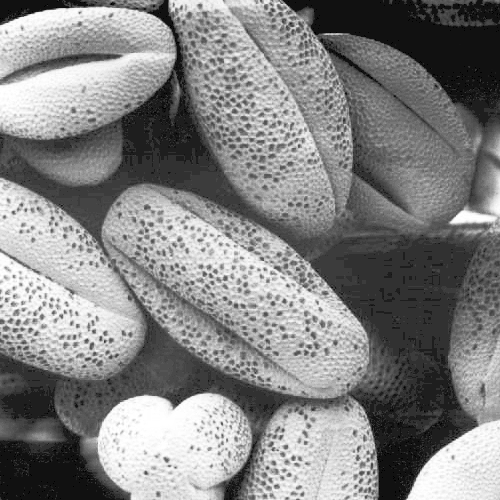
\includegraphics[width=\textwidth]{RESULTADOS/img35.png}
		\caption{Figura 3 mejorada.}
		\label{fig:f18}
	\end{minipage}
	
	\vskip\baselineskip
	
	\begin{minipage}{0.5\textwidth}
		\centering
		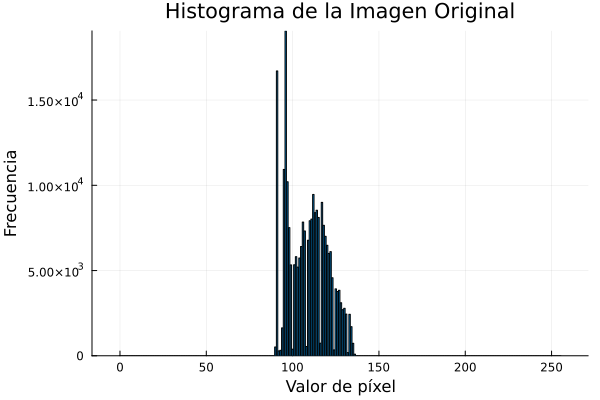
\includegraphics[width=\textwidth]{RESULTADOS/img31.png}
		\caption{Histograma original.}
		\label{fig:f19}
	\end{minipage}\hfill
	\begin{minipage}{0.5\textwidth}
		\centering
		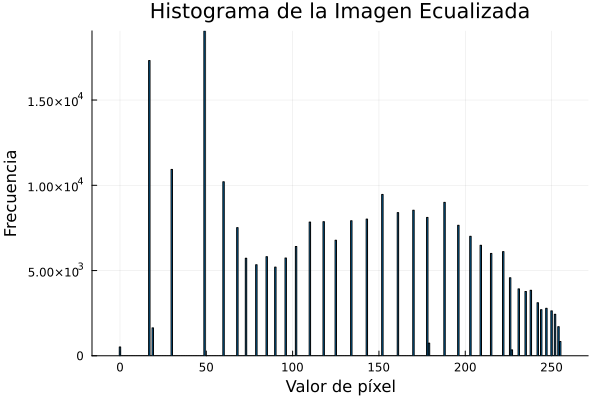
\includegraphics[width=\textwidth]{RESULTADOS/img33.png}
		\caption{Histograma ecualizado.}
		\label{fig:f20}
	\end{minipage}
	\caption{Comparativa de resultados para la figura 3.}
	\label{fig:R5}
\end{figure}

La figura 3 se caracteriza por tener tonos intermedios, ni muy blancos ni muy negros, dicho comportamiento se refleja en su histograma, el cual muestra una concentración de los valores de los pixeles entre 90 y 150 aproximadamente. Dichos comportamiento tiene la particularidad de estar muy compacto hacia el centro de los valores del rango que puede tomar.

Al aplicar la ecualización, la imagen se realza, haciendo una mejor distinción de la figura 3, como si la imagen hubiera sido "limpiada" de polvo que tenia por encima. El histograma asociado muestra como la expansión del rango de los valores de los pixeles se logra, con una mayor carga hacia los valores blancos y siendo muy poco distribuidos los valores de tonos negros que se encuentran entre 0 y 50.

\begin{figure}[htbp]
	\centering
	\begin{minipage}{0.45\textwidth}
		\centering
		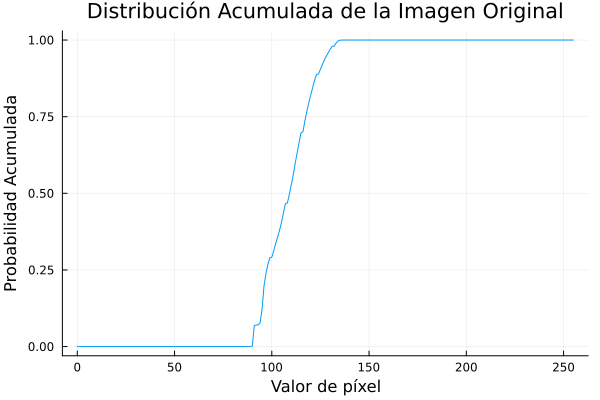
\includegraphics[width=\textwidth]{RESULTADOS/img32.png}
		\caption{Distribución acumulada original.}
		\label{fig:f21}
	\end{minipage}\hfill
	\begin{minipage}{0.45\textwidth}
		\centering
		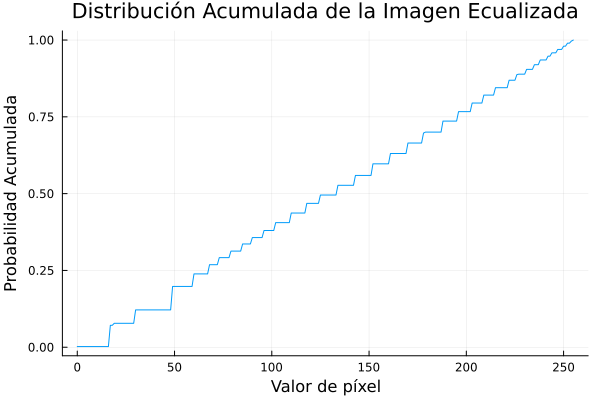
\includegraphics[width=\textwidth]{RESULTADOS/img34.png}
		\caption{Distribución acumulada ecualizada.}
		\label{fig:f22}
	\end{minipage}
	\caption{Comparativa de distribuciones acumuladas para la figura 3.}
	\label{fig:R6}
\end{figure}

Adicionalmente, se hizo el gráfico de la distribución acumulada de probabilidad para la figura 3, dicho gráfico presenta un comportamiento como de función sigmoidal, es decir, tiene un comportamiento casi monotono en los extremos pero es en el centro donde da un salto que la lleva gradualmente de 0 a1 en el intervalo de valores entre 90 y 150.

Al realizar el mejoramiento de la figura, dicha distribución  se regularizada pero con la particularidad de que presenta varias perturbaciones en valores de pixeles entre 0 y 50 que es a donde no termino por expandirse con el histograma.


\newpage
	
\subsection{Figura 4}

\begin{figure}[h]
	\centering
	\begin{minipage}{0.45\textwidth}
		\centering
		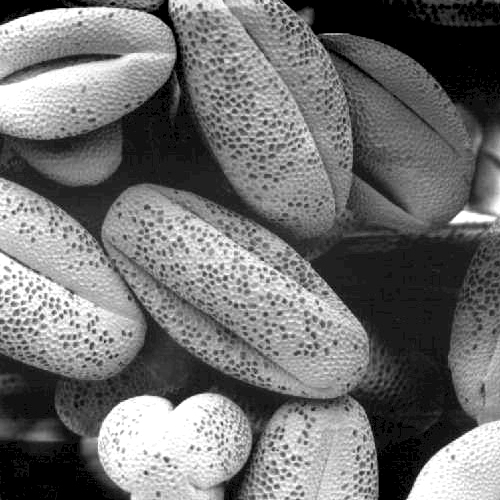
\includegraphics[width=\textwidth]{IMG/Fig3.15(a)4.jpg}
		\caption{Figura 4 original.}
		\label{fig:f23}
	\end{minipage}\hfill
	\begin{minipage}{0.45\textwidth}
		\centering
		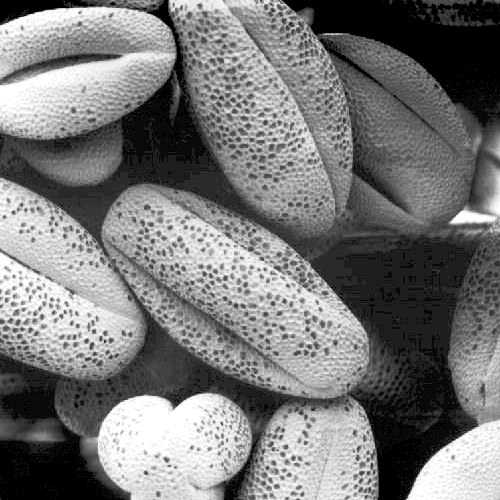
\includegraphics[width=\textwidth]{RESULTADOS/img45.png}
		\caption{Figura 4 mejorada.}
		\label{fig:f24}
	\end{minipage}
	
	\vskip\baselineskip
	
	\begin{minipage}{0.5\textwidth}
		\centering
		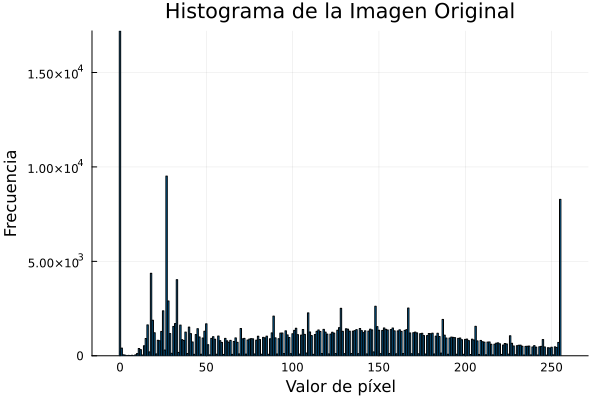
\includegraphics[width=\textwidth]{RESULTADOS/img41.png}
		\caption{Histograma original.}
		\label{fig:f25}
	\end{minipage}\hfill
	\begin{minipage}{0.5\textwidth}
		\centering
		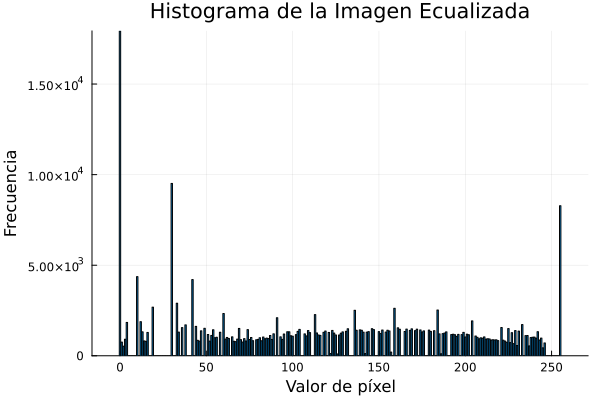
\includegraphics[width=\textwidth]{RESULTADOS/img43.png}
		\caption{Histograma ecualizado.}
		\label{fig:f26}
	\end{minipage}
	\caption{Comparativa de resultados para la figura 4.}
	\label{fig:R7}
\end{figure}

La figura 4 se caracteriza principalmente por ser la más $estándar$, al observar su histograma se puede caer en cuenta del porque se puede decir esto, el histograma muestra una distribución de los valores de los pixeles por todo el rango de  0 a 255 con una carga considerable de valores en negro.

Al aplicar el mejoramiento, a simple vista parece que no cambio mucho, sin emargo, al hacerle zoom a la imagen se pueden apreciar ligeras diferencias entre los matices de los blancos. Por otro lado, el histograma revela que la expansión del rango se mantuvo casí igual a excepción de que ahora hay una mayor distribución de los pixeles entre  0 y 50, rango que no estaba siendo abarcado por la imagen origina.


\begin{figure}[htbp]
	\centering
	\begin{minipage}{0.45\textwidth}
		\centering
		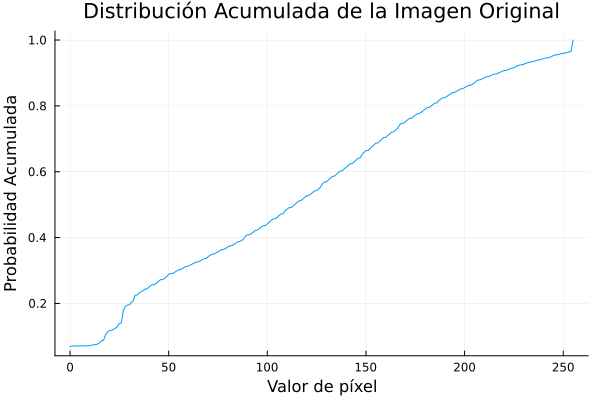
\includegraphics[width=\textwidth]{RESULTADOS/img42.png}
		\caption{Distribución acumulada original.}
		\label{fig:f27}
	\end{minipage}\hfill
	\begin{minipage}{0.45\textwidth}
		\centering
		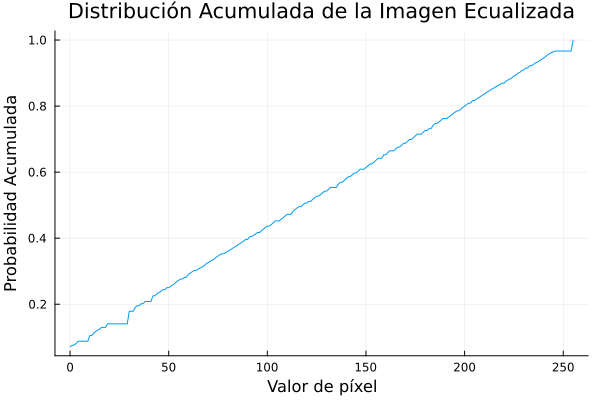
\includegraphics[width=\textwidth]{RESULTADOS/img44.png}
		\caption{Distribución acumulada ecualizada.}
		\label{fig:f28}
	\end{minipage}
	\caption{Comparativa de distribuciones acumuladas para la figura 4.}
	\label{fig:R8}
\end{figure}

Adicionalmente se hizo el gráfico de la distribución de probabilidad acumulada, la cual muestra un comportamiento casi perfecto como diagonal, a excepción de ligeras variaciones, es muy parecida a su versión ecualizada, por lo que a términos prácticos, se traduce en que la imagen si tuvo ciertas mejorías visuales pero son muy sutiles.
	
	
\newpage

	
\section{Conclusiones}
	
Tras la implementación paso a paso y observar los resultados para cada una de las cuatro imagenes, se puede concluir que el mejoramiento por histograma logra su cometido al expandir el rango de valores que pueden tomar los pixeles en una imagen, de forma que queda más uniforme pero con una ligera inclinación hacia los valores donde originalmente estaba más concentrada la distribución. Tal parece que dicha mejora es sustancial en imagenes que los valores de sus pixeles muy compactos, como se vio en el caso de a imagen 1, 2 y 3, en contraposición con el caso de la imagen 4, donde la mejora no fue tan notoria dado que sus pixeles ya estaban repartidos por todo el espacio	


\newpage

	
\section{Referencias}  % Sección numerada de referencias
\bibliographystyle{apalike}  % Estilo de citas (puedes cambiarlo)
\bibliography{Biblio}        % Nombre del archivo BibTeX (sin extensión)

\newpage
	
\section{Anexos}	
\subsection{Implementación de la ecualización por histograma}
\begin{minted}[linenos,firstnumber=1]{julia}
#### Paquetes necesarios ####
using Plots # Para gráficar
using Images # Para manipular imagenes
using StatsBase # Función basicas de estadística

#### Función que hace todo el proceso, genera las gráficas y las imagenes
function ecualizado(img)
	# Convertir la imagen a rango de 0 a 255
	img1 = round.(Int, Gray.(img) .* 255)
	# Obtener la tabla de frecuencias de la imagen original
	tabla = countmap(img1)
	# Definir los niveles de 0 a 255 
	niveles = 0:255
	# Asegurarse de que todos los niveles estén presentes
	tabla1 = Dict(level => get(tabla, level, 0) for level in niveles)
	# Descomponer el resultado en 2 vectores
	x = collect(keys(tabla1))
	y = collect(values(tabla1))
	# Ordenar x y obtener los índices de la ordenación
	indices = sortperm(x)
	# Reordenar x y y según los índices ordenados
	x = x[indices]
	y = y[indices]
	# Calcular las probabilidades
	N = sum(y)  # Total de píxeles
	pp = y / N  # Probabilidad de aparición de cada píxel
	# Acumulador de las probabilidades
	acum = copy(pp)  # Vector de probabilidades para hacer la acumulada
	for i in 2:length(acum)
		acum[i] = acum[i] + acum[i - 1]
	end
	
	# Mostrar el histograma original
	p1 = bar(x, y, label="Histograma Original", legend=:false, 
	xlabel="Valor de píxel", ylabel="Frecuencia",
	title="Histograma de la Imagen Original")
	
	# Mostrar la distribución acumulada original
	p2 = plot(x, acum, label="Distribución Acumulada Original", legend=:false,
	xlabel="Valor de píxel", ylabel="Probabilidad Acumulada",
	title="Distribución Acumulada de la Imagen Original")
	
	# Usar la probabilidad acumulada para asignar el nuevo valor de cada píxel
	imgt = vec(img1)
	
	# Ajuste de los valores de los píxeles
	Fk = round.(255 * acum[imgt .+ 1])  # Fk es el valor ajustado
	F0 = minimum(Fk)  # Valor mínimo ajustado
	salida = round.(255 * ((Fk .- F0) / (255 - F0)))  # Normalizar a [0, 255]
	# Darle el formato original de la matriz
	D = size(img1) # Dimensiones de la imagen
	salida = reshape(salida, D[1], D[2])
	
	# Convertir la matriz a una salida que se rasterice como imagen
	res = clamp.(salida ./ 255, 0, 1)  # Salidas entre 0 y 1
	
	# Mostrar el histograma de la imagen ecualizada
	tabla2 = countmap(round.(Int, res .* 255))  # Conteos ecualizada
	tabla2_ordenada = Dict(level => get(tabla2, level, 0) for level in niveles)
	x2 = collect(keys(tabla2_ordenada))
	y2 = collect(values(tabla2_ordenada))
	# Ordenar en función de los indices
	indices2 = sortperm(x2)
	x2 = x2[indices2]
	y2 = y2[indices2]
	# Proyectar el histograma
	p3 = bar(x2, y2, label="Histograma Ecualizado",
	legend=:false, xlabel="Valor de píxel", 
	ylabel="Frecuencia", title="Histograma de la Imagen Ecualizada")
	
	# Calcular la distribución acumulada de la imagen ecualizada
	N2 = sum(y2)
	pp2 = y2 / N2
	acum2 = copy(pp2)
	for i in 2:length(acum2)
		acum2[i] = acum2[i] + acum2[i - 1]
	end
	
	# Mostrar la distribución acumulada de la imagen ecualizada
	p4 = plot(x2, acum2, 
	label="Distribución Acumulada Ecualizada", legend=:false,
	xlabel="Valor de píxel", ylabel="Probabilidad Acumulada",
	title="Distribución Acumulada de la Imagen Ecualizada")
	# Regresar la imagen ecualizada en formato Gray
	return p1,p2,p3,p4,Gray.(res);
end




#### Lista de rutas de imágenes para las salidas ####

rutas = ["IMG/Fig3.15(a)1.jpg", "IMG/Fig3.15(a)2.jpg",
"IMG/Fig3.15(a)3.jpg", "IMG/Fig3.15(a)4.jpg"]

# Procesar cada imagen y obtener sus salidas #
for (i, ruta) in enumerate(rutas)
	img = load(ruta)
	res = ecualizado(img)
	# Guardar los gráficos y la imagen ecualizada
	savefig(res[1], "RESULTADOS/img$(i)1.png")
	savefig(res[2], "RESULTADOS/img$(i)2.png")
	savefig(res[3], "RESULTADOS/img$(i)3.png")
	savefig(res[4], "RESULTADOS/img$(i)4.png")
	save("RESULTADOS/img$(i)5.png", res[5])
end
\end{minted}

	
	
	
	
	
	
	
\end{document}

